\documentclass[sigconf,anonymous,review]{acmart}

\setcopyright{none}
\settopmatter{printacmref=true,printfolios=true}
\renewcommand\footnotetextcopyrightpermission[1]{}
\acmConference[WWW '27]{The ACM Web Conference 2027}{TBD}{Dublin, Ireland}
\acmBooktitle{The ACM Web Conference 2027 (WWW '27), TBD, Dublin, Ireland}
\acmYear{2027}
\acmDOI{}
\acmISBN{}

\usepackage{booktabs}
\usepackage{multirow}
\usepackage{microtype}
\usepackage{xcolor}
\usepackage{amsmath}
\usepackage{enumitem}
\usepackage{url}
\usepackage{xspace}
\usepackage{tikz}
\usetikzlibrary{arrows.meta,calc,fit,positioning}

\newcommand{\method}{\textsc{STLA}\xspace}
\newcommand{\mapk}{\mathrm{MAP}@100}
\newcommand{\R}{\mathcal{R}}
\newcommand{\A}{\mathcal{A}}
\newcommand{\Pset}{\mathcal{P}}
\newcommand{\wmap}{\mathrm{WorstMAP}@100}
\definecolor{lightblue}{RGB}{235,244,252}
\definecolor{lightgreen}{RGB}{237,248,240}
\definecolor{lightgold}{RGB}{255,248,226}
\definecolor{dediffgreen}{RGB}{151,183,91}
\definecolor{dediffgreenfill}{RGB}{241,247,226}
\definecolor{dediffblue}{RGB}{112,185,207}
\definecolor{dediffbluefill}{RGB}{231,246,250}
\definecolor{dedifforange}{RGB}{241,139,87}
\definecolor{dedifforangefill}{RGB}{255,242,233}
\definecolor{dediffgold}{RGB}{224,172,35}
\definecolor{dediffgoldfill}{RGB}{255,248,220}

\begin{document}

\title{STLA: Backbone-Agnostic, Subgroup-Safe Temporal Logit Adaptation for Web Information Diffusion}

\author{Anonymous Author(s)}
\affiliation{\institution{Anonymous Institution}}

\begin{abstract}
Microscopic information diffusion prediction ranks the next adopter of a social-Web cascade. In deployment, however, user popularity and activity drift over time: yesterday's hubs can become dormant, users absent from historical activity can emerge within a fixed candidate vocabulary, and a model selected on one period can suppress already-retrievable tail or inactive users in the next. We present \method, a 3,517-parameter, backbone-agnostic temporal logit adapter for frozen diffusion predictors. It conditions a low-dimensional score residual on past-only environment summaries, causal prefix descriptors, and five interpretable candidate features. Zero initialization makes the untrained adapter exactly reproduce its anchor, while validation may select epoch zero as an explicit no-regression fallback. A deterministic hierarchical union then preserves every protected candidate retrieved by the anchor at each of $K\in\{10,50,100\}$; we prove the nested-prefix guarantee and audit it exactly. Development experiments across four chronological Web diffusion datasets, two strong graph/hypergraph backbones, and five paired seeds yield non-negative mean $\mapk$ changes in all eight cells, with seven improving in all seeds. Most importantly, we freeze all checkpoints and evaluation code before a one-shot test on an independently prepared, sealed MemeTracker split. \method improves DyHGCN from $0.09868$ to $0.10631$ and DisenIDP from $0.08846$ to $0.09781$ $\mapk$; both mean and worst-period gains are positive in all five seeds ($p=0.03125$). Across the confirmatory test, 1,790/6,055/10,554 protected anchor hits at $K=10/50/100$ are retained with zero violations. The guarantee is conditional on anchor retrieval and is not a demographic-fairness claim. Code: \href{https://anonymous.4open.science/r/STLA-BCE4}{anonymous.4open.science/r/STLA-BCE4}.
\end{abstract}

\keywords{information diffusion, temporal distribution shift, ranking, safe adaptation, social Web}

\begin{CCSXML}
<ccs2012>
<concept><concept_id>10002951.10003227.10003351</concept_id><concept_desc>Information systems~Social networks</concept_desc><concept_significance>500</concept_significance></concept>
</ccs2012>
\end{CCSXML}
\ccsdesc[500]{Information systems~Social networks}

\maketitle

\section{Introduction}
\textbf{Web relevance.} Predicting who will next adopt, repost, or propagate information is a core Web task. It supports cascade simulation, content moderation, early trend detection, and capacity planning on social platforms. Modern microscopic predictors combine cascade order, time, social links, graphs, and hypergraphs to rank the next user \cite{li2017deepcas,wang2017topolstm,yuan2020dyhgcn,sun2022mshgat,cheng2023disenidp}. Their usual evaluation assumption is nevertheless static: a model is optimized on historical cascades and its ranking rule is carried forward unchanged.

This assumption is fragile on the Web. Attention shifts, communities reorganize, and the identities of active hubs change. Such temporal drift can invalidate both representations and popularity priors. It has at least two scales. \emph{Environment shift} changes which users are active between chronological blocks; \emph{prefix shift} changes the evidence available as an individual cascade grows. A useful correction must distinguish the two: a single global temperature cannot express candidate-specific popularity change, while a dense per-user correction can memorize development identities and fail to transfer. Our development-only audit later confirms substantial adjacent-window activity churn and low overlap between successive hub sets.

Dynamic graph models evolve embeddings or parameters \cite{pareja2020evolvegcn,kumar2019jodie,trivedi2019dyrep,xu2020tgat}, while concept-drift methods update a predictor as its data distribution changes \cite{gama2014survey,webb2016drift}. Both directions usually assume access to a particular backbone state or to observations from the period being adapted to. For next-user diffusion, a practical deployment update must instead satisfy three requirements simultaneously: it should work with heterogeneous frozen predictors, condition only on information available before the target environment, and avoid silently deleting useful retrieval for tail, inactive, or emerging candidates.

The last requirement is subtle. A regularizer can improve an average metric while moving an already-correct protected target below a product cutoff. Fair-ranking research offers prefix, representation, and exposure constraints \cite{zehlike2017fair,celis2018ranking,biega2018equity,singh2018exposure}, but our setting is different: group labels are behavioral and time-varying, not demographic; the desired contract is the preservation of particular anchor items rather than parity. We therefore seek a small temporal correction with an exact, auditable ranking invariant.

We propose \method. It treats any frozen diffusion predictor as a logit-producing anchor. For each chronological environment, a past-only encoder summarizes cumulative and recent user activity and graph degree. For each cascade prefix, a causal descriptor determines five coefficients that score historical popularity, recent popularity, popularity change, dormancy, and emergence. This yields a rank-five residual over users without reading a backbone hidden state. The factorization is deliberately asymmetric: candidate statistics contain the identities of \emph{effects}, while the learned network predicts only five effect strengths. Its 3,517 parameters therefore do not scale with the user vocabulary.

Two safeguards turn this adapter into a conservative update. First, the final layer is initialized to zero and epoch zero participates in validation selection, making the frozen anchor an executable fallback rather than a conceptual baseline. Second, at inference a hierarchical protected union restores protected anchor items at $K=10,50,100$ while retaining the adaptive order elsewhere. The two mechanisms address different risks: fallback prevents a globally harmful validation choice, whereas fusion prevents item-level protected regressions even when the adapted ranking improves on average.

Our evaluation separates development from confirmation. Four chronological diffusion datasets are used only for validation-based method development. We then independently prepare MemeTracker \cite{leskovec2009memetracking}, prevent the selection loader from materializing its test file, hash all selected artifacts, and open the test payload once. This paper makes five contributions:

\begin{itemize}[leftmargin=*,itemsep=1pt,topsep=2pt]
  \item a backbone-agnostic, 3,517-parameter temporal score adapter using only past environments and observed cascade prefixes;
  \item a deterministic multi-cutoff fusion rule with a nested-prefix preservation proof and exact violation audit;
  \item a chronological evaluation design that separates past-only feature construction, validation-only development, and an independently sealed one-shot test;
  \item five-seed evidence on two architecturally distinct anchors across four development datasets, including explicit epoch-zero and mixed-effect boundaries; and
  \item a sealed MemeTracker test showing significant mean and worst-period gains for both anchors while preserving every protected anchor hit.
\end{itemize}

\noindent\textbf{Scope.} The task, data, and failure mode are intrinsically Web-centered: the candidate universe is a social-platform user graph, inputs are time-stamped online cascades, and the output is a ranked next-adopter list under evolving online attention. We do not merely apply a generic learner to social-network data; the method's past-only temporal environments and multi-cutoff preservation contract are designed for Web diffusion rankings.

\section{Related Work}
\subsection{Microscopic diffusion prediction}
Microscopic diffusion prediction asks \emph{who} will propagate next rather than only how large a cascade will become. DeepCas aggregates random-walk cascade paths \cite{li2017deepcas}, TopoLSTM couples topology with recurrent sequence modeling \cite{wang2017topolstm}, and DeepDiffuse jointly models adopter identity and timing \cite{islam2018deepdiffuse}. Hawkes-inspired methods such as DeepHawkes connect predictive representations to self-exciting diffusion dynamics \cite{cao2017deephawkes}, while CasFlow explicitly represents hierarchical propagation uncertainty \cite{xu2023casflow}.

Graph and hypergraph predictors then make user relations more explicit. DyHGCN constructs dynamic heterogeneous graphs to encode changing user preferences \cite{yuan2020dyhgcn}; MS-HGAT uses sequential hypergraphs and memory \cite{sun2022mshgat}; and DisenIDP separates user and cascade representations with self-supervision \cite{cheng2023disenidp}. These methods improve the backbone representation itself. \method addresses a different lifecycle stage: after an expensive predictor has been trained and frozen, it adapts only the exposed user logits. This distinction makes one temporal mechanism applicable to DyHGCN and DisenIDP without aligning their incompatible hidden states.

\subsection{Temporal drift and dynamic graphs}
Temporal graph learning represents evolving interactions through recurrent states, point processes, attention, or parameter evolution \cite{kazemi2020dynamic}. JODIE projects user and item trajectories \cite{kumar2019jodie}; DyRep couples representation updates with event intensities \cite{trivedi2019dyrep}; EvolveGCN changes graph-convolution parameters across snapshots \cite{pareja2020evolvegcn}; and TGAT uses functional time encodings for inductive temporal attention \cite{xu2020tgat}. TGN unifies memory, message, and embedding modules \cite{rossi2020tgn}, causal anonymous walks capture temporal motifs \cite{wang2021caw}, while GraphMixer and DyGFormer explore simpler pooling and long-history Transformer designs \cite{cong2023graphmixer,yu2023dygformer}.

These methods are powerful when one can redesign or continually execute the temporal backbone. They do not directly solve frozen-model maintenance across graph, hypergraph, and sequential architectures. Moreover, recent benchmarks show that temporal split design, repeated edges, negative sampling, and real-world time shift can dominate apparent gains \cite{poursafaei2022better,huang2023tgb,yao2022wildtime}. Our setting is neither ordinary snapshot prediction nor online target-stream updating: each query is an ordered cascade prefix, activity changes between chronological environments, and no aggregate from the target environment is admissible. We therefore place the temporal mechanism outside the backbone and construct it from a strict past filtration.

\subsection{Distribution shift, calibration, and adaptation}
Concept drift describes changes in a stream's generating process and motivates detection, forgetting, and adaptation \cite{gama2014survey,webb2016drift}; domain-adaptation theory formalizes the difficulty of transferring between different source and target distributions \cite{bendavid2010domains}. Post-hoc calibration instead transforms outputs of a fixed predictor. Temperature and related scaling methods can improve probability estimates with very few parameters \cite{niculescu2005probabilities,guo2017calibration}, but a single class-independent scale cannot express that dormant and newly popular users should move in opposite directions.

Test-time adaptation methods such as Tent, MEMO, CoTTA, and EATA update model parameters from unlabeled target inputs \cite{wang2021tent,zhang2022memo,wang2022cotta,niu2022eata}. Their stability and model selection can be sensitive under dynamic streams \cite{niu2023sar,zhao2023pitfalls}. That access pattern is deliberately excluded here: even unlabeled activity from a future Web period leaks which users became active. \method is closer to structured logit calibration, but conditions candidate-separable corrections on \emph{preceding} environments and selects them on an ordinary validation block. It therefore does not claim source-free or fully test-time adaptation; its contribution is a no-lookahead interface for frozen diffusion rankings.

\subsection{Safe and fair ranking}
Ranking interventions have addressed representation, exposure, and utility under group constraints. FA*IR enforces prefix-wise protected representation \cite{zehlike2017fair}; constrained-ranking formulations study quality under multiple prefix bounds \cite{celis2018ranking}; and exposure-based objectives distribute attention across items or groups \cite{biega2018equity,singh2018exposure}. Other work designs database ranking schemes or operational rerankers for search and recommendation \cite{asudeh2019designing,geyik2019fairness}; complementary surveys organize score-based and learning-to-rank fairness definitions \cite{zehlike2022survey,zehlike2022survey2}.

Our guarantee is narrower and deterministic. It does not assert demographic parity, equal exposure, or retrieval of a target missed by the anchor. It guarantees that if a behaviorally protected item lies in an anchor prefix, it remains in the same fused prefix. This preservation contract is appropriate when temporal adaptation may improve a frozen production ranking but must not erase its existing protected successes. Table~\ref{tab:position} summarizes this positioning.

\begin{table*}[t]
\caption{Positioning of \method relative to representative neighboring approaches. ``Target-period access'' means that unlabeled events or aggregate statistics from the deployment period are consumed during adaptation.}
\label{tab:position}
\centering
\scriptsize
\begin{tabular}{@{}p{2.4cm}p{3.9cm}p{2.5cm}p{2.2cm}p{2.0cm}p{2.5cm}@{}}
\toprule
Line of work & Representative methods & What changes & Target-period access & Frozen-logit interface & Item-wise anchor-hit guarantee\\
\midrule
Diffusion prediction & DeepCas, DyHGCN, MS-HGAT, DisenIDP & Backbone representation and objective & Not required at inference & No & No\\
Temporal graph learning & JODIE, TGAT, TGN, CAW, GraphMixer & Temporal states, attention, or backbone parameters & Often consumes events up to query time & No & No\\
Post-hoc calibration & Probability and temperature scaling & Output scores & Calibration split & Yes & No\\
Test-time adaptation & Tent and related source-free updates & Normalization or model parameters & Yes, unlabeled target batches & Usually no & No\\
Fair reranking & FA*IR, exposure and constrained-ranking methods & Ranked list or ranking policy & Depends on setting & Yes & Group/exposure constraints, not this contract\\
\method & Past-conditioned temporal logit residual plus union & Five coefficients and final ranking & \textbf{No}; preceding environments only & \textbf{Yes} & \textbf{Yes}, at $K=10,50,100$\\
\bottomrule
\end{tabular}
\end{table*}

\section{Problem and Protocol}
Let $\mathcal{U}$ be the set of candidate users. A cascade is a time-stamped sequence $c=(u_1,t_1),\ldots,(u_m,t_m)$. Given prefix $c_{1:i}$, a frozen anchor $f$ produces logits $\mathbf{z}^{A}_{i}\in\mathbb{R}^{|\mathcal U|}$ for next user $u_{i+1}$. Cascades are sorted by start time and divided into tie-preserving chronological train, validation, and test blocks.

We further partition train into four environments and validation into two; the independent test uses three environments. Let $\mathcal F_{<e}$ be the information filtration generated by cascades whose start times precede environment $e$. An admissible temporal feature must be measurable with respect to $\mathcal F_{<e}$. Operationally, every environment statistic is computed from $\mathcal H_e\subset\mathcal F_{<e}$, and every query statistic uses only the observed prefix $c_{1:i}$. Neither target labels, unlabeled cascades, user counts, nor aggregate activity from $e$ enter the adapter. Hit and MAP use real users only; padding and end-of-sequence tokens cannot be targets.

The prediction goal is to improve the chronological utility of the frozen anchor without violating a conditional preservation contract. For cutoff $K$, let $A_K(c_{1:i})$ denote the anchor prefix, $F_K(c_{1:i})$ the final prefix, and $G_e(v)\in\{0,1\}$ a past-only behavioral protection indicator. The required set is
\begin{equation}
P_K(c_{1:i})=\{v\in A_K(c_{1:i}):G_e(v)=1\}.
\end{equation}
The contract is $P_K(c_{1:i})\subseteq F_K(c_{1:i})$ for every query and every requested $K\in\{10,50,100\}$. It is conditional because $P_K$ contains only items already retrieved by the anchor. This separates the learned objective (future next-user accuracy) from the deployment invariant (no loss of an existing protected hit).

We distinguish two evidence tiers. \emph{Development evidence} uses validation only; no test dataset, tensor, or model input is constructed. It supports architecture choices, ablations, and transfer diagnostics but not a one-shot claim. \emph{Confirmatory evidence} uses an independently prepared test split after selection, code, and hashes are frozen. This division follows the broader lesson from temporal-graph benchmarking that chronology and evaluation design are part of the method rather than incidental preprocessing \cite{poursafaei2022better,huang2023tgb}. Exact one-sided paired sign-flip tests operate on five seed-wise differences. With five non-zero pairs, the smallest attainable $p$ is $2^{-5}=0.03125$.

\subsection{Metrics and paired inference}
Each next-user query has one relevant target. If its rank is $r$, then $\mathrm{AP}@K=1/r$ for $r\le K$ and zero otherwise. We average queries within each chronological environment, then report the unweighted mean of environment MAPs. This environment macro-average prevents a longer time block from dominating the temporal conclusion. We define $\wmap$ as the minimum environment $\mapk$; it measures the observed worst block rather than adversarial robustness. Hit@$K$ is defined analogously without reciprocal-rank discount.

All comparisons pair the same five seeds between an anchor and its adapted result. For seed-wise deltas $\delta_1,\ldots,\delta_5$, the exact one-sided sign-flip test enumerates all $2^5$ sign assignments and counts assignments whose mean is at least the observed mean. Zero deltas are retained in the enumeration. We report effect sizes, the number of strictly positive pairs, and $p$ together because the small paired sample makes significance alone uninformative.

\section{Method}
Figure~\ref{fig:pipeline} summarizes \method. The anchor is frozen throughout.

\begin{figure*}[t]
\centering
\resizebox{\textwidth}{!}{%
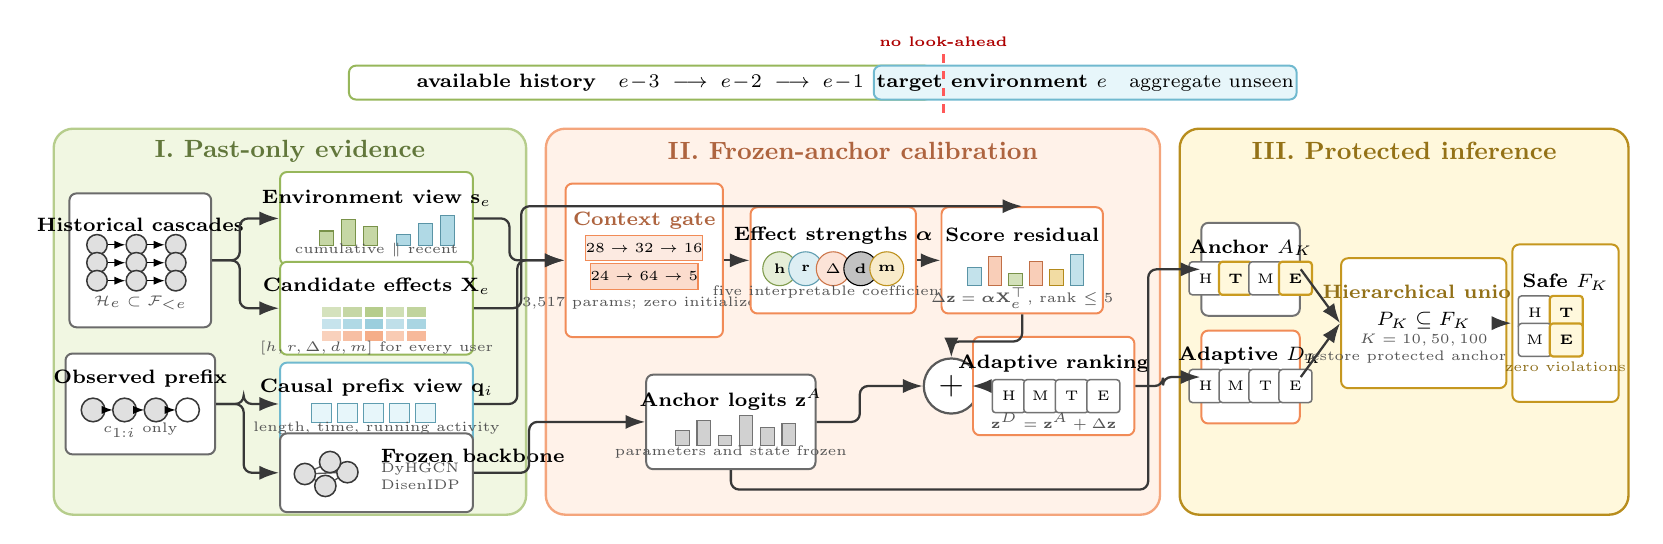
\begin{tikzpicture}[
  x=1cm,y=.76cm,
  flow/.style={-{Latex[length=2.5mm,width=1.8mm]},line width=0.82pt,draw=black!78},
  softflow/.style={flow,rounded corners=3pt},
  panel/.style={draw=black!58,fill=white,line width=0.72pt,rounded corners=2.5pt,align=center,font=\scriptsize,inner sep=2.5pt},
  stage/.style={font=\small\bfseries,align=center},
  label/.style={font=\scriptsize\bfseries,align=center},
  sublabel/.style={font=\tiny,align=center,text=black!67},
  dot/.style={circle,draw=black!78,fill=black!12,line width=.55pt,minimum size=3.5mm,inner sep=0pt,font=\tiny},
  protected/.style={rectangle,draw=dediffgold!90!black,fill=dediffgoldfill,line width=.8pt,rounded corners=1.2pt,minimum width=4.2mm,minimum height=4.2mm,inner sep=0pt,font=\tiny\bfseries},
  ordinary/.style={rectangle,draw=black!55,fill=white,line width=.55pt,rounded corners=1.2pt,minimum width=4.2mm,minimum height=4.2mm,inner sep=0pt,font=\tiny}
]
% Three semantic regions: graphical objects first, text second.
\path[draw=dediffgreen!70,fill=dediffgreenfill,line width=.85pt,rounded corners=7pt]
  (-.35,-3.20) rectangle (5.65,3.25);
\path[draw=dedifforange!78,fill=dedifforangefill,line width=.85pt,rounded corners=7pt]
  (5.90,-3.20) rectangle (13.70,3.25);
\path[draw=dediffgold!82!black,fill=dediffgoldfill,line width=.85pt,rounded corners=7pt]
  (13.95,-3.20) rectangle (19.65,3.25);

\node[stage,text=dediffgreen!65!black] at (2.65,2.88)
  {I. Past-only evidence};
\node[stage,text=dedifforange!72!black] at (9.80,2.88)
  {II. Frozen-anchor calibration};
\node[stage,text=dediffgold!66!black] at (16.80,2.88)
  {III. Protected inference};

% Chronology ribbon.
\node[panel,draw=dediffgreen,fill=white,minimum width=7.4cm,minimum height=.43cm,inner sep=1pt]
  (historybar) at (7.10,4.02)
  {\textbf{available history}\quad $e\!-\!3\;\longrightarrow\;e\!-\!2\;\longrightarrow\;e\!-\!1$};
\node[panel,draw=dediffblue,fill=dediffbluefill,minimum width=3.05cm,minimum height=.43cm,inner sep=1pt]
  (targetbar) at (12.75,4.02) {\textbf{target environment $e$}\quad aggregate unseen};
\draw[dashed,red!65,line width=.85pt] (10.95,3.52) -- (10.95,4.52);
\node[font=\tiny\bfseries,text=red!68!black,above] at (10.95,4.46) {no look-ahead};

% Stage I: cascade icons and compact multi-view objects.
\node[panel,minimum width=1.80cm,minimum height=1.70cm] (hist) at (.75,1.05) {};
\node[label] at (.75,1.65) {Historical cascades};
\foreach \yy in {1.31,1.01,.71}{
  \node[dot,minimum size=2.6mm] at (.20,\yy) {};
  \node[dot,minimum size=2.6mm] at (.70,\yy) {};
  \node[dot,minimum size=2.6mm] at (1.20,\yy) {};
  \draw[-{Latex[length=1.4mm]},line width=.5pt] (.34,\yy)--(.56,\yy);
  \draw[-{Latex[length=1.4mm]},line width=.5pt] (.84,\yy)--(1.06,\yy);
}
\node[sublabel] at (.75,.34) {$\mathcal H_e\subset\mathcal F_{<e}$};

\node[panel,minimum width=1.90cm,minimum height=1.28cm] (seq) at (.75,-1.35) {};
\node[label] at (.75,-.92) {Observed prefix};
\foreach \x in {.15,.55,.95}{\node[dot,minimum size=3mm] at (\x,-1.45) {};}
\node[dot,minimum size=3mm,fill=white] at (1.35,-1.45) {};
\draw[-{Latex[length=1.4mm]},line width=.55pt] (.30,-1.45)--(.40,-1.45);
\draw[-{Latex[length=1.4mm]},line width=.55pt] (.70,-1.45)--(.80,-1.45);
\draw[-{Latex[length=1.4mm]},line width=.55pt] (1.10,-1.45)--(1.20,-1.45);
\node[sublabel] at (.75,-1.79) {$c_{1:i}$ only};

\node[panel,draw=dediffgreen,minimum width=2.45cm,minimum height=1.18cm] (env) at (3.75,1.75) {};
\node[label] at (3.75,2.09) {Environment view $\mathbf s_e$};
\foreach \x/\h/\c in {3.02/.24/dediffgreen,3.30/.43/dediffgreen,3.58/.31/dediffgreen,4.00/.18/dediffblue,4.28/.36/dediffblue,4.56/.50/dediffblue}{
  \path[draw=\c!80!black,fill=\c!55,line width=.4pt] (\x,1.30) rectangle +(0.18,\h);
}
\node[sublabel] at (3.75,1.23) {cumulative $\Vert$ recent};

\node[panel,draw=dediffgreen,minimum width=2.45cm,minimum height=1.18cm] (cand) at (3.75,.25) {};
\node[label] at (3.75,.62) {Candidate effects $\mathbf X_e$};
\foreach \x/\s in {3.05/40,3.32/55,3.59/70,3.86/45,4.13/60}{
  \path[draw=white,line width=.3pt,fill=dediffgreen!\s] (\x,.10) rectangle +(0.25,.18);
  \path[draw=white,line width=.3pt,fill=dediffblue!\s] (\x,-.10) rectangle +(0.25,.18);
  \path[draw=white,line width=.3pt,fill=dedifforange!\s] (\x,-.30) rectangle +(0.25,.18);
}
\node[sublabel] at (3.75,-.42) {$[h,r,\Delta,d,m]$ for every user};

\node[panel,draw=dediffblue,minimum width=2.45cm,minimum height=1.05cm] (pref) at (3.75,-1.35) {};
\node[label] at (3.75,-1.08) {Causal prefix view $\mathbf q_i$};
\foreach \x in {3.05,3.38,3.71,4.04,4.37}{
  \node[rectangle,draw=dediffblue!85!black,fill=dediffbluefill,minimum width=2.5mm,minimum height=2.5mm,inner sep=0pt] at (\x,-1.50) {};
}
\node[sublabel] at (3.75,-1.75) {length, time, running activity};

\node[panel,draw=black!58,minimum width=2.45cm,minimum height=1.00cm] (anchor) at (3.75,-2.50) {};
\node[label,anchor=west] at (3.68,-2.22) {Frozen backbone};
\draw[line width=.48pt,black!65] (2.84,-2.52)--(3.10,-2.72)--(3.38,-2.49)--(3.16,-2.32)--cycle;
\draw[line width=.48pt,black!65] (2.84,-2.52)--(3.38,-2.49);
\foreach \x/\y in {2.84/-2.52,3.10/-2.72,3.38/-2.49,3.16/-2.32}{
  \node[dot,minimum size=2.7mm] at (\x,\y) {};
}
\node[sublabel,anchor=west,align=left] at (3.68,-2.56) {DyHGCN\\DisenIDP};

\draw[softflow] (hist.east) -- ++(.35,0) |- (env.west);
\draw[softflow] (hist.east) -- ++(.35,0) |- (cand.west);
\draw[softflow] (seq.east) -- ++(.35,0) |- (pref.west);
\draw[softflow] (seq.east) -- ++(.35,0) |- (anchor.west);

% Stage II: one compact learned path plus the untouched anchor path.
\node[panel,draw=dedifforange,fill=white,minimum width=2.00cm,minimum height=1.95cm] (gate) at (7.15,1.05) {};
\node[label,text=dedifforange!72!black] at (7.15,1.72) {Context gate};
\node[rectangle,draw=dedifforange,fill=dedifforange!18,minimum width=1.35cm,minimum height=3.2mm,inner sep=0pt,font=\tiny] at (7.15,1.26) {$28\to32\to16$};
\node[rectangle,draw=dedifforange,fill=dedifforange!30,minimum width=1.05cm,minimum height=3.2mm,inner sep=0pt,font=\tiny] at (7.15,.78) {$24\to64\to5$};
\node[sublabel] at (7.15,.34) {3,517 params; zero initialized};

\node[panel,draw=dedifforange,minimum width=2.10cm,minimum height=1.35cm] (alpha) at (9.55,1.05) {};
\node[label] at (9.55,1.47) {Effect strengths $\boldsymbol\alpha$};
\foreach \x/\t/\c in {8.87/h/dediffgreen,9.20/r/dediffblue,9.55/$\Delta$/dedifforange,9.90/d/black,10.23/m/dediffgold}{
  \node[circle,draw=\c!85!black,fill=\c!24,minimum size=4.3mm,inner sep=0pt,font=\tiny\bfseries] at (\x,.91) {\t};
}
\node[sublabel] at (9.55,.52) {five interpretable coefficients};

\node[panel,draw=dedifforange,minimum width=2.05cm,minimum height=1.35cm] (res) at (11.95,1.05) {};
\node[label] at (11.95,1.47) {Score residual};
\foreach \x/\h/\c in {11.26/.30/dediffblue,11.52/.48/dedifforange,11.78/.20/dediffgreen,12.04/.40/dedifforange,12.30/.27/dediffgold,12.56/.52/dediffblue}{
  \path[draw=\c!80!black,fill=\c!42,line width=.4pt] (\x,.63) rectangle +(0.17,\h);
}
\node[sublabel] at (11.95,.42) {$\Delta\mathbf z=\boldsymbol\alpha\mathbf X_e^\top$, rank $\le5$};

\node[panel,draw=black!58,minimum width=2.15cm,minimum height=1.20cm] (alogit) at (8.25,-1.65) {};
\node[label] at (8.25,-1.28) {Anchor logits $\mathbf z^A$};
\foreach \x/\h in {7.55/.25,7.82/.42,8.09/.18,8.36/.50,8.63/.30,8.90/.38}{
  \path[draw=black!55,fill=black!18,line width=.4pt] (\x,-2.05) rectangle +(0.17,\h);
}
\node[sublabel] at (8.25,-2.16) {parameters and state frozen};

\node[circle,draw=black!65,fill=white,line width=.8pt,minimum size=7mm,inner sep=0pt,font=\large] (plus) at (11.05,-1.05) {$+$};
\node[panel,draw=dedifforange,minimum width=2.05cm,minimum height=1.25cm] (adaptive) at (12.35,-1.05) {};
\node[label] at (12.35,-.68) {Adaptive ranking};
\node[ordinary] at (11.78,-1.22) {H};
\node[ordinary] at (12.18,-1.22) {M};
\node[ordinary] at (12.58,-1.22) {T};
\node[ordinary] at (12.98,-1.22) {E};
\node[sublabel] at (12.35,-1.65) {$\mathbf z^D=\mathbf z^A+\Delta\mathbf z$};

\draw[softflow] (env.east) -- ++(.45,0) |- (gate.west);
\draw[softflow] (pref.east) -- ++(.55,0) |- (gate.west);
\draw[flow] (gate) -- (alpha);
\draw[flow] (alpha) -- (res);
\draw[softflow] (cand.east) -- ++(.60,0) |- (res.north);
\draw[softflow] (anchor.east) -- ++(.70,0) |- (alogit.west);
\draw[softflow] (res.south) -- ++(0,-.45) -| (plus.north);
\draw[softflow] (alogit.east) -- ++(.55,0) |- (plus.west);
\draw[flow] (plus) -- (adaptive);

% Stage III: two ranked lists enter a deterministic protected union.
\node[panel,draw=black!55,minimum width=1.25cm,minimum height=1.18cm] (alist) at (14.85,.90) {};
\node[label] at (14.85,1.26) {Anchor $A_K$};
\node[ordinary] at (14.28,.75) {H};
\node[protected] at (14.66,.75) {T};
\node[ordinary] at (15.04,.75) {M};
\node[protected] at (15.42,.75) {E};

\node[panel,draw=dedifforange,minimum width=1.25cm,minimum height=1.18cm] (dlist) at (14.85,-.90) {};
\node[label] at (14.85,-.54) {Adaptive $D_K$};
\node[ordinary] at (14.28,-1.05) {H};
\node[ordinary] at (14.66,-1.05) {M};
\node[ordinary] at (15.04,-1.05) {T};
\node[ordinary] at (15.42,-1.05) {E};

\node[panel,draw=dediffgold!88!black,fill=white,minimum width=2.10cm,minimum height=1.65cm] (union) at (17.05,0) {};
\node[label,text=dediffgold!65!black] at (17.05,.52) {Hierarchical union};
\node[font=\scriptsize] at (17.05,.04) {$P_K\subseteq F_K$};
\node[sublabel] at (17.05,-.43) {$K=10,50,100$\\restore protected anchor hits};

\node[panel,draw=dediffgold!88!black,minimum width=1.35cm,minimum height=2.00cm] (safe) at (18.85,0) {};
\node[label] at (18.85,.68) {Safe $F_K$};
\node[ordinary] at (18.46,.18) {H};
\node[protected] at (18.86,.18) {T};
\node[ordinary] at (18.46,-.28) {M};
\node[protected] at (18.86,-.28) {E};
\node[sublabel,text=dediffgold!62!black] at (18.85,-.72) {zero violations};

\draw[flow] (alist.east) -- (union.west);
\draw[flow] (dlist.east) -- (union.west);
\draw[flow] (union) -- (safe);
\draw[softflow] (adaptive.east) -- ++(.35,0) |- (dlist.west);
\draw[softflow] (alogit.south) -- (8.25,-2.78) -- (13.55,-2.78) -- (13.55,.90) -- (alist.west);

\end{tikzpicture}%
}
\caption{The \method framework, organized into three semantic regions. Past cascades and the observed prefix form compact environment, candidate, and prefix views. A zero-initialized 3,517-parameter gate produces a rank-five residual on top of frozen anchor logits. The deterministic union then restores protected tail or emerging items (gold $T/E$) at every requested cutoff.}
\label{fig:pipeline}
\Description{A three-stage graphical pipeline. Green panels show historical cascades, a cumulative-versus-recent environment chart, and a candidate-effect matrix; a blue sequence supplies a causal prefix view and a frozen DyHGCN or DisenIDP anchor. In the orange stage, a compact context gate emits five interpretable coefficients, multiplies them by candidate effects, and adds the score residual to frozen anchor logits. In the gold stage, anchor and adaptive top-K lists enter a hierarchical protected union, producing safe prefixes in which protected tail and emerging items are restored at cutoffs 10, 50, and 100.}
\end{figure*}

\subsection{Past-only environment and candidate features}
For cumulative history and the most recent preceding window, we summarize user popularity and graph degree with 14 statistics: active fraction and count; mean, standard deviation, maximum, median, and 90th percentile of log popularity; Gini coefficient; normalized entropy; top-1\% and top-5\% popularity mass; and the mean, standard deviation, and maximum of log degree. Concatenating the two views yields $\mathbf s_e\in\mathbb R^{28}$. The recent view responds to short-lived attention shifts, whereas the cumulative view provides a stable scale when a recent window is sparse. A two-layer encoder maps their concatenation to context $\mathbf h_e\in\mathbb R^{16}$.

Every candidate $v$ receives five features derived from $\mathcal H_e$:
\begin{equation}
\mathbf x_{e,v}=[\bar p^{\mathrm{hist}}_v,\bar p^{\mathrm{recent}}_v,
\bar p^{\mathrm{recent}}_v-\bar p^{\mathrm{hist}}_v,d_v,m_v],
\end{equation}
where the first two terms are standardized $\log(1+p)$ counts, $d_v$ marks historical-but-currently-dormant users, and $m_v$ marks users unseen in history.

Table~\ref{tab:features} makes the residual semantics explicit. Standardization is recomputed from $\mathcal H_e$ and applied to the fixed candidate vocabulary; it never uses the target block. The change feature is the difference of two standardized quantities rather than a raw count difference, preventing high-volume datasets from dominating coefficient scale. Dormancy and emergence remain binary because their operational meaning is categorical.

\begin{table}[t]
\caption{Five candidate effects in $\mathbf X_e$. A positive coefficient increases candidates with larger feature values; the learned sign may vary by environment and prefix.}
\label{tab:features}
\centering
\small
\begin{tabular}{@{}lp{3.35cm}p{3.2cm}@{}}
\toprule
Symbol & Past-only definition & Behavioral interpretation\\
\midrule
$\bar p^{\mathrm{hist}}$ & standardized cumulative $\log(1+p)$ & established popularity\\
$\bar p^{\mathrm{recent}}$ & standardized recent $\log(1+p)$ & current momentum\\
$\Delta\bar p$ & $\bar p^{\mathrm{recent}}-\bar p^{\mathrm{hist}}$ & rising or fading attention\\
$d$ & historical $>0$, recent $=0$ & dormant user\\
$m$ & historical $=0$ & emerging-in-history user\\
\bottomrule
\end{tabular}
\end{table}

For position $i$, an eight-dimensional prefix vector $\mathbf q_i$ contains relative log prefix length, a bounded transform of elapsed duration, running means and maxima of historical and recent log popularity, and the fractions of dormant and emerging users already observed. These features tell the gate whether the current cascade is short or mature and whether its observed adopters already depart from historical activity. All running quantities use $c_{1:i}$ only and are updated causally as $i$ advances.

\subsection{Backbone-agnostic residual}
A gated MLP maps $[\mathbf h_e;\mathbf q_i]$ to five coefficients $\boldsymbol\alpha_{e,i}$. The adaptive logits are
\begin{equation}
\mathbf z^{D}_{e,i}=\mathbf z^A_i+\boldsymbol\alpha_{e,i}\mathbf X_e^\top,
\label{eq:residual}
\end{equation}
where row $v$ of $\mathbf X_e$ is $\mathbf x_{e,v}$. The environment encoder is $28\to32\to16$ and the gate is $24\to64\to5$, with LayerNorm, GELU, and dropout. Counting weights, biases, and normalization parameters gives $1{,}544+1{,}973=3{,}517$ trainable parameters, independent of $|\mathcal U|$. There is no learned user embedding or per-dataset output head.

The factorization is low rank in candidate space. For two users $v,w$,
\begin{equation}
|\Delta z_{e,i,v}-\Delta z_{e,i,w}|
\le \|\boldsymbol\alpha_{e,i}\|_2\,\|\mathbf x_{e,v}-\mathbf x_{e,w}\|_2.
\label{eq:sensitivity}
\end{equation}
Thus the adapter can reorder users only through five declared behavioral axes. Equation~\ref{eq:sensitivity} is not a generalization bound, but it exposes a useful stability mechanism: users with similar historical and recent behavior receive similar corrections regardless of identity. It also permits an audit of which coefficients caused a change.

\subsection{Training, selection, and exact fallback}
The anchor is evaluated under \texttt{no\_grad}; only the adapter receives gradients. For each valid next-user target we minimize cross entropy of $\mathbf z^D$ with Adam, gradient clipping, and weight decay. Training batches alternate chronological training environments so that the same gate observes multiple past-to-future transitions. The final gate layer is initialized to zero, hence $\boldsymbol\alpha=\mathbf 0$ and $\mathbf z^D=\mathbf z^A$ exactly before the first update.

After every epoch we evaluate the hierarchical-union ranking on validation and retain the checkpoint with the highest mean validation $\mapk$. Epoch zero is serialized and participates in this ordinary selection rule. Once selected, the adapter, anchor, manifest, and evaluator are frozen; no online gradient or target-period statistic is used during confirmation.

\begin{proposition}[Validation fallback]
Let $M$ be the fused validation selection metric and let epoch zero be among the candidate checkpoints. Then the selected checkpoint satisfies $M_{\mathrm{selected}}\ge M_{\mathrm{anchor}}$ on validation.
\end{proposition}
\begin{proof}
Zero initialization gives identical adaptive and anchor logits. Every required protected item is already present, so hierarchical union performs no membership replacement and returns the anchor order. Epoch zero therefore attains $M_{\mathrm{anchor}}$; maximizing over a set that includes it cannot select a lower value.
\end{proof}

This proposition is deliberately validation-scoped. It prevents optimization from forcing a known validation regression, but it does not imply that a nonzero adapter will improve every future dataset. The Android epoch-zero selections are an empirical example of this boundary.

\subsection{Hierarchical protected union}
Past-only popularity labels use four groups: the top 20\% of previously active users are head, the next 30\% are mid, the remainder are tail, and zero-history users are emerging. Recency labels are recent-active, historical-inactive, and emerging. We protect every non-head or non-recent candidate. Let $A_K$ and $D_K$ be the anchor and adaptive top-$K$ lists, and let $P_K\subseteq A_K$ contain protected anchor items. Starting from the adaptive top-100 list, we process $K=10,50,100$. Missing items in $P_K$ are swapped forward if already present, otherwise they replace the lowest-ranked non-required item in the current prefix. The resulting list is $F$.

Concretely, for each cutoff the algorithm (1) scans the corresponding anchor prefix in anchor order; (2) forms the required set from past-only labels; (3) identifies required users absent from the current fused prefix; and (4) allocates slots from the bottom upward. If a missing user already occurs later in the adaptive top-100 list, a swap preserves both membership and uniqueness. Otherwise the user replaces the lowest-ranked item not required at the current cutoff. Processing cutoffs in increasing order is essential: a single top-100 union does not guarantee that a protected top-10 item remains in the final top 10.

\begin{proposition}[Nested-prefix preservation]
For every requested $K\in\{10,50,100\}$, $P_K\subseteq F_K$ and $F_K$ contains no duplicates.
\end{proposition}
\begin{proof}
At cutoff $K$, $|P_K|\le K$, so the prefix has enough positions. A missing required item either swaps with its unique later occurrence or replaces a position occupied by an item outside $P_K$; both operations preserve uniqueness and terminate with $P_K\subseteq F_K$. Because anchor prefixes are nested, $P_{10}\subseteq P_{50}\subseteq P_{100}$. Later passes never replace a current-prefix item belonging to their required set, which includes every earlier required item. Thus induction over increasing cutoffs preserves all established guarantees.
\end{proof}

The proposition is a ranking invariant, not a statistical fairness statement. It guarantees a protected target remains hit only when the anchor already hits it at that cutoff. It also preserves the adaptive ordering of every pair never touched by a swap or replacement; the empirical accuracy cost of the touched positions is measured rather than assumed away.

\subsection{Design rationale and complexity}
Equation~\ref{eq:residual} factorizes the correction into five prefix-conditioned coefficients and five candidate features. A dense learned per-user residual would add parameters tied to a particular vocabulary and could memorize development identities. Our factorization keeps trainable size independent of $|\mathcal U|$, exposes the sign of each popularity/recency effect, and lets a new dataset reuse the same interface. The environment vector is separate from the cascade-prefix vector because the former changes once per chronological block while the latter changes at every next-user position.

For $B$ prediction positions and $N$ candidates, residual construction costs $O(5BN)$ arithmetic and stores the ordinary $B\times N$ logit matrix already required for ranking. Candidate statistics cost $O(N)$ per environment and are cached. Given the two top-100 lists, hierarchical fusion processes at most 100 candidates per prediction; its list-processing cost is $O(100)$ and independent of the backbone graph or hypergraph. Top-$K$ extraction shares the same $O(BN)$ score scan already required by ranking evaluation. Zero initialization is more than a training heuristic: it makes adapter construction, checkpoint serialization, and validation fallback verifiable by exact tensor and ranking equality.

\section{Experiments}
\subsection{Data and temporal splitting}
Experimental tables report ratios as percentages ($\times100$) and omit cell-level \% signs; counts and $p$-values keep native units. The compact release omits a decimal point in timestamps; inserting it after the first six digits makes all retained cascades nondecreasing. We retain lengths 5--500, remap users, and construct a tie-preserving 70/10/20 split. The strict selection loader opens only train and validation; a unit test replaces the test JSON with invalid bytes and confirms loader construction still succeeds.

Counts in Table~\ref{tab:data} refer to real users in the available processed bundle, not padding/EOS vocabulary entries. Because the corrected chronological protocol and candidate semantics differ from earlier experimental pipelines, we treat these runs as controlled development comparisons rather than reproductions of prior tables. MemeTracker is prepared independently and used for confirmation. The same 70/10/20 chronological rule is applied throughout; split-boundary timestamp ties move together rather than being divided across periods.

\begin{table}[t]
\caption{Chronological datasets. ``Dev'' results are validation-only; MemeTracker supplies the sealed test.}
\label{tab:data}
\centering
\small
\begin{tabular}{lrrrl}
\toprule
Dataset & Users & Cascades & Train/Val/Test & Role\\
\midrule
Christianity & 1,651 & 589 & 412/59/118 & Dev\\
Android & 2,927 & 678 & 475/67/136 & Dev\\
Douban & 12,232 & 3,475 & 2,432/348/695 & Dev\\
Twitter & 12,627 & 3,435 & 2,404/344/687 & Dev\\
MemeTracker & 4,709 & 10,130 & 7,091/1,013/2,026 & Sealed test\\
\bottomrule
\end{tabular}
\end{table}

\subsection{Development-only temporal shift audit}
Before choosing the adapter, we quantify whether the four development datasets actually exhibit changes that a static popularity prior can miss. We divide each train-plus-validation prefix into six equal-count windows and compare adjacent windows. Jensen--Shannon (JS) divergence measures change in the user-adoption distribution; hub Jaccard is the overlap between the top 20\% active users; and active-user churn is one minus Jaccard overlap of all active users. These diagnostics use no test split and never become model inputs.

\begin{table}[t]
\caption{Adjacent-window drift on train plus validation only (mean over five transitions). Lower hub overlap and higher JS/churn indicate stronger temporal change.}
\label{tab:drift}
\centering
\small
\begin{tabular}{lrrr}
\toprule
Dataset & JS divergence & Hub Jaccard & Active churn\\
\midrule
Christianity & 27.9 & 48.2 & 61.3\\
Android & 28.3 & 31.6 & 47.7\\
Douban & 31.0 & 39.1 & 65.8\\
Twitter & 34.0 & 32.9 & 57.1\\
\bottomrule
\end{tabular}
\end{table}

Table~\ref{tab:drift} shows that drift is not merely a motivating anecdote. Successive top-hub sets overlap by only 0.316--0.482 on average, while 47.7--65.8\% of the active-user set turns over between adjacent windows. Twitter has the largest mean JS divergence, whereas Douban has the largest active-user churn. The measures need not agree because probability mass can move among a stable active set, or many low-frequency users can churn without dominating mass. This distinction motivates combining distribution summaries with candidate-level recent and historical activity rather than relying on one scalar drift score.

\subsection{Backbones and training}
We use corrected implementations of DyHGCN \cite{yuan2020dyhgcn} and DisenIDP \cite{cheng2023disenidp}, selected by validation $\mapk$ and then frozen. These architectures respectively emphasize dynamic heterogeneous graph convolution and self-supervised disentangled hypergraph representations. Their distinct internal states test the output-only interface. We also retrain MS-HGAT \cite{sun2022mshgat} for five seeds under the same chronological split and matched optimizer. All three model implementations are pinned community integrations rather than exact author-official reproductions. We additionally evaluate three deterministic past-only rankings: cumulative popularity, most-recent-window popularity, and their standardized difference (momentum). The adapter uses context dimension 16, hidden dimension 64, environment hidden dimension 32, dropout 0.2, batch size 64, Adam learning rate $10^{-3}$, weight decay $10^{-4}$, and at most ten epochs. Seeds are 21, 42, 84, 126, and 168.

``Corrected'' denotes protocol and metric repairs rather than a new backbone: the runner selects on validation instead of testing every epoch, excludes padding/EOS from the candidate space, masks previously observed cascade users according to the task semantics, and constructs temporal graph inputs only from preceding cascades. The frozen anchor exposes real-user logits but no hidden representation to the adapter. This common interface is important because DyHGCN and DisenIDP have incompatible internal graph operators and state layouts.

For each validation partition, two chronological environments define worst-period performance; the sealed MemeTracker test uses three. Every seed reuses the same split and pairs its adapted checkpoint with the corresponding anchor checkpoint. We report mean $\pm$ sample standard deviation over paired seeds, the number of positive differences, relative effect size, and exact one-sided sign-flip $p$-values. No claim is based only on the seed-21 run. Hyperparameters are fixed across both anchors; only the selected epoch varies.

\noindent\textbf{Evaluation questions.}
We organize the evidence around four questions: \textbf{RQ1} does adaptation improve an untouched future period; \textbf{RQ2} does the effect transfer across backbones and datasets; \textbf{RQ3} which components matter and what accuracy cost buys the preservation contract; and \textbf{RQ4} are the safety and confirmatory claims directly auditable?

\subsection{Independent one-shot MemeTracker test}
Figure~\ref{fig:results} is the primary result. Before opening the test payload, we froze SHA-256 values for ten anchor checkpoints, ten adapters, their selection records, the split manifest, evaluator source, and test file. The evaluator verifies every hash and refuses to overwrite an existing seed result.

\begin{figure*}[t]
  \centering
  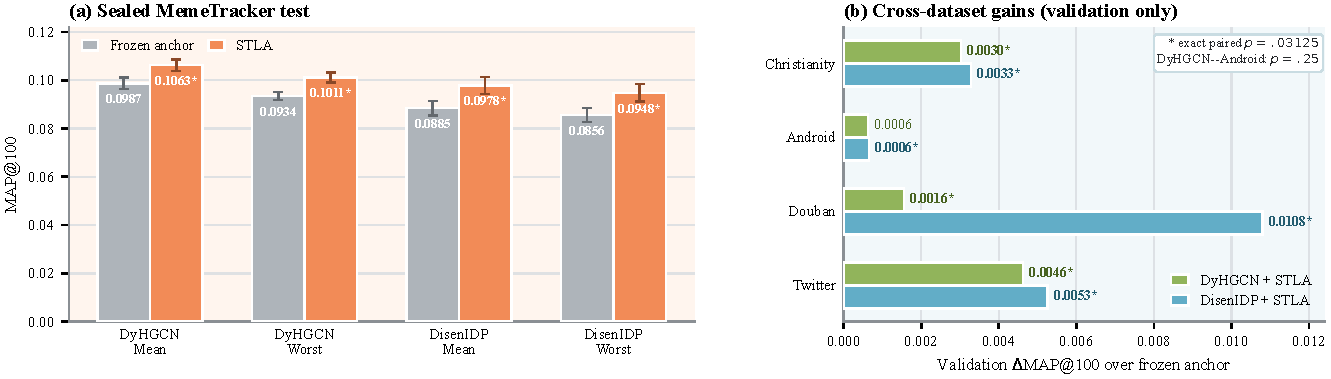
\includegraphics[width=\textwidth]{figures/result_comparison.pdf}
  \caption{Visual comparison of the main experimental effects. (a) On the sealed one-shot MemeTracker test, \method improves both mean and worst-period MAP@100 for two frozen anchors; error bars are sample standard deviations over five paired seeds, and the zero-based axis avoids magnifying the differences. (b) Validation-only gains over the same frozen anchors on four development datasets. $^{*}$ marks an exact one-sided paired sign-flip test at $p=0.03125$; DyHGCN--Android is the sole nonsignificant mean comparison ($p=0.25$).}
  \Description{Two-panel result chart. The left panel compares frozen-anchor and STLA MAP at 100 on the sealed MemeTracker test for DyHGCN and DisenIDP, showing higher STLA bars for mean and worst-period metrics. The right panel shows positive validation gains on Christianity, Android, Douban, and Twitter, with DyHGCN on Android marked nonsignificant.}
  \label{fig:results}
\end{figure*}

On the sealed test, \method raises DyHGCN mean and worst-period $\mapk$ by $0.00764$ and $0.00765$ (7.74\% and 8.19\%), and DisenIDP by $0.00935$ and $0.00914$ (10.57\% and 10.67\%). All four comparisons improve in 5/5 seeds and attain the minimum exact $p=0.03125$; Table~\ref{tab:paired} exposes every paired delta in the prespecified seed order. The effect also holds at $K=10,50,100$ for both anchors (Figure~\ref{fig:diagnostics}c); near-flat gains from 50 to 100 locate most useful reorderings in the high-utility part of the list.

\begin{table}[t]
\caption{Adapted-minus-anchor $\mapk$ / $\wmap$ on sealed MemeTracker. Values are percentage-point differences.}
\label{tab:paired}
\centering
\small
\begin{tabular}{rcc}
\toprule
Seed & DyHGCN & DisenIDP\\
\midrule
21  & 0.550 / 0.541 & 0.430 / 0.405\\
42  & 0.748 / 0.749 & 1.061 / 0.951\\
84  & 0.817 / 0.722 & 0.987 / 1.020\\
126 & 0.711 / 0.768 & 1.154 / 1.069\\
168 & 0.994 / 1.048 & 1.045 / 1.123\\
\bottomrule
\end{tabular}
\end{table}

\subsection{Cross-dataset development evidence}
Table~\ref{tab:dev} broadens the comparison to eight methods spanning three nonparametric rankings, MS-HGAT, two strong anchors, and their adapted variants. Recent popularity is the strongest heuristic on all four datasets, yet remains below the best learned result; MS-HGAT is competitive on Christianity and Android but trails DyHGCN on Douban and Twitter. The gain is therefore not an artifact of comparing only with a weak static model.

Against the two strongest scalable anchors, all eight \method cells have non-negative mean deltas, seven improve in all five seeds, and seven attain $p=0.03125$ (Figure~\ref{fig:results}b). DyHGCN--Android is the explicit mean boundary: two seeds improve and three select epoch zero ($p=0.25$). Worst-period gains are consistent in six cells, while DisenIDP--Android is mixed; we do not claim universal worst-period improvement.

This is a controlled comparison, not a paper-by-paper leaderboard: learned rows share data, chronological boundaries, prefix cap, masking, matched optimizer, and evaluator, but community integrations and preprocessing preclude claims of exact author-official reproduction. Statistical marks compare only paired anchor--adapter runs. On Christianity, Android, Douban, and Twitter, the strongest adapted value exceeds the strongest unadapted learned row by $0.00328$, $0.00066$, $0.00156$, and $0.00463$, respectively.

MemeTracker validation independently follows the same direction: DyHGCN moves from $0.11940\pm0.00325$ to $0.12237\pm0.00346$, and DisenIDP from $0.10672\pm0.00372$ to $0.11160\pm0.00337$. Both mean and worst-period comparisons improve in 5/5 paired seeds at $p=0.03125$; these values select the adapters before the sealed test is opened and are never pooled with its effect. Twitter and Douban show consistent gains amid high drift, whereas Android's substantial hub turnover yields small mean effects; aggregate drift motivates maintenance but does not predict every backbone--dataset response.

\begin{table*}[t]
\caption{Development baselines (validation-only MAP@100). Learned rows report five-seed mean $\pm$ sample standard deviation; $^{*}$ marks an exact one-sided paired improvement over its frozen anchor ($p=0.03125$).}
\label{tab:dev}
\centering
\scriptsize
\begin{tabular}{@{}llcccc@{}}
\toprule
Family & Method & Christianity & Android & Douban & Twitter\\
\midrule
\multirow{3}{*}{Nonparametric}
 & Cumulative popularity & 6.472 & 1.685 & 4.202 & 0.388\\
 & Recent popularity & 7.360 & 1.867 & 4.596 & 1.235\\
 & Popularity momentum & 1.818 & 0.161 & 3.757 & 0.728\\
\midrule
Sequential hypergraph & MS-HGAT & $9.275\pm0.144$ & $2.772\pm0.076$ & $4.637\pm0.088$ & $2.751\pm0.684$\\
\midrule
\multirow{2}{*}{Graph anchor}
 & DyHGCN & $8.818\pm0.260$ & $2.620\pm0.185$ & $5.836\pm0.125$ & $18.354\pm0.502$\\
 & DyHGCN + \method & $9.120^{*}\pm0.169$ & $2.683\pm0.132$ & $\mathbf{5.992}^{*}\pm0.141$ & $\mathbf{18.817}^{*}\pm0.621$\\
\midrule
\multirow{2}{*}{Hypergraph anchor}
 & DisenIDP & $9.485\pm0.139$ & $2.772\pm0.046$ & $4.380\pm0.143$ & $12.916\pm0.306$\\
 & DisenIDP + \method & $\mathbf{9.813}^{*}\pm0.160$ & $\mathbf{2.838}^{*}\pm0.070$ & $5.460^{*}\pm0.097$ & $13.442^{*}\pm0.372$\\
\bottomrule
\end{tabular}
\end{table*}

\begin{figure*}[t]
  \centering
  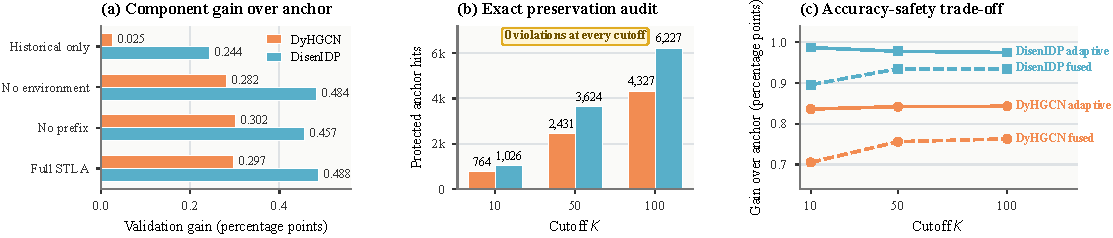
\includegraphics[width=\textwidth]{figures/diagnostic_panels.pdf}
  \caption{Diagnostic comparisons. (a) Validation-only component gains. (b) Sealed-test protected anchor-hit opportunities (zero violations). (c) Sealed-test MAP@$K$ gains before (solid) and after (dashed) fusion; the 0.040--0.131-point cost keeps all gains positive.}
  \Description{Three-panel diagnostic chart. The first panel shows validation gains for four component configurations and two backbones. The second shows increasing protected-hit counts at cutoffs 10, 50, and 100 with zero violations. The third shows that adaptive and safely fused rankings both remain above their anchors at all three cutoffs.}
  \label{fig:diagnostics}
\end{figure*}

\subsection{Post-confirmation component analysis}
Figure~\ref{fig:diagnostics}a is deliberately separated from the untouched test result. After confirmation was complete, we trained 30 additional adapters against MemeTracker train/validation only; the loader again did not materialize test data. ``Historical only'' retains the environment and prefix conditioning but restricts the five candidate features to historical popularity. The other variants remove one context source while retaining all candidate features.

Restricting candidate evidence to historical popularity loses $0.00273$ and $0.00244$ versus full \method; full is higher in all five paired seeds for both anchors ($p=0.03125$). Environment context adds a small, consistent $0.00015$ for DyHGCN (5/5) but is neutral for DisenIDP. Prefix removal is mixed and nearly neutral. Thus the richer temporal candidate statistics drive most of the validation effect, while the two context sources provide modest, architecture-dependent refinement. We do not claim every component is uniformly necessary. Every ablation still has zero preservation violations because fusion enforces the invariant independently of calibration features.

This ablation separates two claims that are easy to conflate. Candidate features are the main empirical source of improvement; environment and prefix context determine when those effects should change. The latter two are not uniformly necessary on one validation dataset, so the present evidence supports a compact conditional parameterization rather than a claim that all 28 environment and eight prefix dimensions are individually indispensable. A preregistered future comparison can test whether the simpler no-prefix form transfers, but it cannot retroactively change the sealed result reported here.

\subsection{Preservation audit}
For each prediction and cutoff, an opportunity is counted when the true next user is behaviorally protected and lies in the frozen anchor top-$K$; a violation occurs if that target is absent from the fused top-$K$. The audit therefore tests the proposition at target level, not only aggregate group exposure. Figure~\ref{fig:diagnostics}b reports the sealed test: all 1,790 top-10, 6,055 top-50, and 10,554 top-100 opportunities are retained. The four-dataset development audit adds 6,150, 13,569, and 17,931 opportunities, respectively. Across both tiers and backbones, the exact audit finds zero violations. This does not imply equal numbers of arbitrary protected candidates in the adaptive and fused lists; the invariant is item-specific and anchor-conditional.

\subsection{Accuracy cost of the safety layer}
Figure~\ref{fig:diagnostics}c separates the learned adaptive ranking from deterministic fusion on the sealed test. The unrestricted adapter achieves the highest MAP, while fusion gives up $0.00040$--$0.00131$ absolute MAP depending on cutoff and backbone. Crucially, the fused ranking remains well above the anchor at every cutoff. The contract therefore has a measurable, small cost rather than being presented as free. At $K=100$, fusion retains 90.6\% of DyHGCN's unrestricted gain and 95.9\% of DisenIDP's.

\section{Integrity, Reproducibility, and Limitations}
Even unlabeled target-period activity can leak which users become popular. Features therefore use only $\mathcal F_{<e}$; timestamp ties remain intact; selection loaders expose only train/validation paths and survive invalid test bytes; padding/EOS and observed prefix users are excluded according to the declared candidate semantics; and serialized epoch zero participates in validation selection.

Before test materialization we record hashes for chronological splits, selected anchor and adapter checkpoints, selection results, evaluator source, and the sealed payload. The evaluator verifies every entry before its first read, opens the test once, evaluates the fixed $2\times5$ backbone--seed pairs, writes immutable pair-level JSON, refuses missing entries or overwrite, and emits the complete summary. No test-derived value changes a checkpoint, feature, hyperparameter, cutoff, or claim definition.

MemeTracker preparation retains 10,130 of 10,131 raw cascades, 4,709 users, and 77,126 directed edges. The selected manifest digest is \texttt{68b753d91ca2...c2de}; all 63 pre-freeze unit tests pass. Released evidence includes the split manifest, checkpoint/result hashes, all ten one-shot results, exact summarizer, and protected-hit audit. Code and hashes support computational reproducibility; inaccessible test data and immutable outputs support confirmatory integrity. These controls make the narrow claim auditable but do not make MemeTracker representative of every platform.

\subsection{Limitations and ethical scope}
The exact sign-flip test supports a paired directional claim, not a population-level estimate over arbitrary datasets or platforms. Evidence is deliberately narrow: one independent dataset, five seeds, and coarse exact-test resolution. The other datasets and post-confirmation component analysis are validation-only; Android shows that worst-period gains are not universal, and the ablations cannot retroactively strengthen the sealed claim. Chronological blocks must be fixed before evaluation: abrupt within-block drift may require finer environments, while overly fine blocks make past statistics noisy.

The emerging indicator denotes a user absent from history but already present in the fixed vocabulary, not a newly created account; serving new accounts requires an inductive backbone. Engineered activity signals also exclude semantic, policy, and exogenous shocks. Preservation is anchor-conditional, not demographic fairness: it cannot recover a protected target absent from the anchor top-$K$, and restoring one may replace an unprotected adaptive item. Behavioral groups may correlate with sensitive attributes, and popularity can encode exposure feedback; past-only construction prevents leakage, not confounding. Figure~\ref{fig:diagnostics}c measures ranking cost but not every product utility affected by an exchange. Deployment additionally requires platform-specific policy review, privacy and abuse controls, score-change limits, and exposure and content-quality monitoring.

\section{Conclusion}
\method turns temporal maintenance of frozen diffusion predictors into a small, separately testable output layer. Its five-factor residual uses only preceding environments and observed cascade prefixes; zero initialization preserves an exact validation fallback, and hierarchical union protects every behaviorally designated anchor hit at the requested cutoffs.

Across four development datasets and two distinct backbones, all eight mean effects are non-negative and seven are significant; Android prevents a universal-gain claim. On sealed MemeTracker, both backbones improve mean and worst-period $\mapk$ in every paired seed and at $K=10,50,100$, with zero preservation violations.

This evidence supports past-only improvement without target-period activity or deletion of protected successes; future work should test inductive candidates and exposure constraints on additional Web platforms.

\clearpage

\bibliographystyle{ACM-Reference-Format}
\bibliography{references}

\end{document}
